\RequirePackage{etex} 

\documentclass[12pt,a4paper]{amsart}

\usepackage{accents}
\usepackage{cleveref}
\usepackage{fullpage}
\usepackage{graphicx}
\usepackage{macros}
\usepackage{mathtools}
\usepackage{natbib}

\theoremstyle{remark}
\newtheorem{example}{Example}

\title{Seminar 1}
\author{Giovanni Pistone}
\date{\today}

\begin{document}

\maketitle

\section{Introduction}

In \citet*{raus|elshiaty|petra:arXiv2401.05196}, the authors suggest using the exponential geometry of exponential families but expressing it in the mixture coordinates. See the classical monograph \citet*{brown:86} for exponential families. About infinite dimensional exponential families, see \citet*{pistone:2013gsi}. Here, we rephrase the same ideas and applications in the language on statistical bundles according to \citet*{chirco|pistone:2022}.

\section{Examples}
\label{sec:examples}

\subsection{Poisson}

The Poisson probability function (PF) is
\begin{equation}
  \label{eq:1}
  p(y,\eta) = \frac{\eta^y}{y!} \euler^{-\eta}, \text{with $y \in \posintegers$ and $\eta \in ]0,+\infty[$},
\end{equation}
that is, the log-PF is
\begin{equation}
  \label{eq:20}
  \log p(y;\eta) = (\log \eta) y - \eta - \log y! \ .
\end{equation}

If we change the $\eta$ parameter to $\theta = \log \eta$, that is, $\theta \in \reals$, then $\euler^\theta = \eta$ and
\begin{equation}
  \label{eq:2}
  p(y;\euler^{\theta}) = \frac{\euler^{\theta y}}{y!} \euler^{-\euler^\theta} = \expof{\theta y - \log y! - \euler\theta} =\expof{\theta y - (\euler^{\theta} - 1)} p(y;1) \ .
\end{equation}

The equation above is an exponential family in the reference $p_1$. The parameter $\theta$ is the natural parameter for the sufficient statistics $u \colon y \to y$. The cumulant function is
\begin{equation}
  \label{eq:3}
  \psi(\theta) = \euler^\theta - 1 \ , \quad \text{with} \quad \text{$\psi'(\theta) = \euler^{\theta} = \eta$ and $\psi''(\theta) = \euler^\theta  = \eta$}.
\end{equation}

In the non-parametric point of view, the \cref{eq:2} is the exponential family $\expmodat V$ generated by the affine space $V = \spanof{u,1}$, $u \colon \posintegers \ni y \mapsto y \in \reals$. It is a sub-model of the maximal exponential family $\maxexpat {p_1}$.

The fibre at $p_\eta$ of the statistical bundle $\expbundleat {V}$ is
\begin{equation}
  \label{eq:5}
    \expfibreat {p_\eta} {V} = \spanof{u - \eta} = \setof{\xi(u-\eta)}{\xi \in \reals} \ .
  \end{equation}
Notice that we distinguish between the model parameters and the coordinates in the fibre as the points are PFs, and the random variables in the fibre are velocities.

The covariance inner product on the fibre at $p_\eta$ is 
\begin{multline}
  \label{eq:8}
  \expfibreat {p_\eta} {V} \times \expfibreat {p_\eta} {V} \ni (\xi_1(u - \eta),\xi_2(u-\eta)) \mapsto \\ \covat {p_\eta}{\xi_1(u - \eta)}{\xi_2(u-\eta)} = \xi_1\xi_2 \expectat {p_\eta} {(u - \eta)^2} = \eta\,\xi_1\xi_2\ .
\end{multline}
Compare with \cref{eq:3}.

See in \citet*{chirco|pistone:2022} the construction of the affine exponential geometry of the open probability simplex via the definition of exponential displacement. In the natural parameter, the exponential displacement of the Poisson exponential family is
\begin{multline}
  \label{eq:6}
  (\theta_1,\theta_2) \mapsto \left(p_{\euler^{\theta_1}},p_{\euler^{\theta_2}}\right) \mapsto S_{p_{\euler^{\theta_1}}}(p_{\euler^{\theta_2}}) = \log \frac {p_{\euler^{\theta_2}}}{p_{\euler^{\theta_1}}} - \expectat {p_{\euler^{\theta_1}}} {\log \frac {p_{\euler^{\theta_2}}}{p_{\euler^{\theta_1}}}} = \\ (\theta_2 - \theta_1) u - (\euler^{\theta_2} - \euler^{\theta_1}) - \expectat {p_{\euler^{\theta_1}}} {(\theta_2 - \theta_1) u - (\euler^{\theta_2} - \euler^{\theta_1})} = \\  (\theta_2-\theta_1) (u - \euler^{\theta_1}) \mapsto \theta_2 - \theta_1 = S_{\theta_1}(\theta_2) \ ,
\end{multline}
while in the expectation parameter, the exponential displacement is
\begin{equation}
  \label{eq:9}
  (\eta_1,\eta_2) \mapsto (p_{\eta_1},p_{\eta_2}) \mapsto S_{p_{\eta_1}}(p_{\eta_2}) = \log \frac {\eta_2}{\eta_1} (u - \eta_1) \mapsto \log \frac {\eta_2}{\eta_1} = S_{\eta_1}(\eta_2) \ .
\end{equation}

Notice that the variance of the displacement in its fibre is a divergence,
\begin{equation}
  \label{eq:22}
  \expectat {p_{\eta_1}} {\left(S_{p_{\eta_1}}(p_{\eta_2})\right)^2} =  \expectat {p_{\eta_1}} {\left(\log \frac {\eta_2}{\eta_1} (u - \eta_1)\right)^2} = \left(\log \frac {\eta_2}{\eta_1}\right)^2 \eta_1 \ .  
\end{equation}

The exponential parallel transport is
\begin{equation}
  \label{eq:10}
  \etransport {p_{\eta_1}} {p_{\eta_2}} \colon \expfibreat {p_{\eta_1}} {V} \ni \xi(u - \eta_1) \mapsto \xi(u - \eta_2) \in \expfibreat {p_{\eta_2}} V \ ,
\end{equation}
that is, is the identity in the $\xi$-coordinates, $\etransport {\eta_1}{\eta_2} \xi = \etransport {\theta_1}{\theta_2} \xi = \xi$.

The parallelogram law for the exponential displacement is 
\begin{equation}
  \label{eq:11}
  S_{p_{\eta_1}}(p_{\eta_2}) + \etransport {p_{\eta_2}}{p_{\eta_1}} S_{p_{\eta_2}}(p_{\eta_3}) = S_{p_{\eta_1}}(p_{\eta_3}) \ ,
\end{equation}
that is,
\begin{equation}
  \label{eq:12}
  \log \frac {\eta_2}{\eta_1}(u - \eta_1) + \log \frac {\eta_3}{\eta_2} \etransport {p_{\eta_2}}{p_{\eta_1}} (u - \eta_2) = \log \frac {\eta_3}{\eta_1}  (u - \eta_1) \ . 
\end{equation}

The velocity of the curve $\eta \mapsto p_\eta$ is
\begin{equation}
  \label{eq:13}
  \derivby \eta \log p_\eta = \derivby \eta (\log \eta u - \eta - \log u!) = \frac 1 \eta u - 1  
\end{equation}
and the velocity of the curve $\theta \mapsto p_{\euler^\theta}$ is 
\begin{equation}
  \label{eq:14}
  \derivby \theta \log p_{\euler^\theta} = \derivby \theta (\theta u - \euler^\theta - \log u!) = \left(\frac 1 {\euler^\theta} u - 1\right) \euler^\theta = u - \euler^\theta \ . 
\end{equation}

The curve $t \mapsto q(t) = p_{\eta(t)}$ is an exponential geodesic with initial velocity $\xi (u - \eta)$ at $\eta(0) = \eta$ if the velocity is constant up to the exponential transport,
\begin{equation}
  \label{eq:15}
  \derivby t \log p_{\eta(t)} = \left(\frac 1 {\eta(t)} u - 1\right) \dot \eta(t) = \frac {u - \eta(t)} {\eta(t)} \dot \eta(t)=  \xi (u - \eta(t)) \ ,  
\end{equation}
that is,
\begin{equation}
  \label{eq:16}
  \frac {\dot \eta(t)} {\eta(t)} = \derivby t \log \eta(t) = \xi \ , \quad  \eta(0) = \eta \ .
\end{equation}

It follows $\log \eta(t) = \log \eta + t \xi$, so that
\begin{equation}
  \label{eq:17}
  \log q(t) = \log \eta(t)u - \eta(t) - u! = (\log \eta + t \xi) u - \euler^{\eta + t \xi} - \log u! \ . 
\end{equation}
The initial conditions are satisfied. Notice that $\theta(t) = \log \eta(t) = \log \eta + t \xi$, that is, $t \mapsto \theta(t)$ is an affine function of $t$.

\subsubsection{Dual parallel transport}
Let us compute the dual $\mtransport {}{}$ of the e-transport $\etransport {}{}$. For each $\xi_1(u - \eta_1) \in \expfibreat {p_{\eta_1}} V$ and $\xi_2(u - \eta_2) \in \expfibreat {p_{\eta_2}} V$,
\begin{equation}
  \label{eq:4}
  \scalarat {p_{\eta_2}} {\etransport {p_{\eta_1}}{p_{\eta_2}} \xi_1(u - \eta_1)} {\xi_2(u - \eta_2)} = \xi_1 \xi_2 \expectat {p_{\eta_2}} {(u - \eta_2)^2} =  \eta_2\,\xi_1 \xi_2 \ .
\end{equation}
We look for a $\widehat{\xi}_2$ such that
\begin{equation}
  \label{eq:7}
   \eta_2 \xi_1\xi_2 = \scalarat {p_{\eta_1}} {\xi_1(u - \eta_1)}{\widehat{\xi}_2(u - \eta_1)} = \eta_1 \xi_1 \widehat{\xi}_2 \ ,
\end{equation}
namely, $\widehat{\xi}_2 = \frac {\eta_2}{\eta_1} \xi_2$. In conclusion, the dual (or mixture) transport is
\begin{equation}
  \label{eq:18}
  \mtransport {p_{\eta_2}}{p_{\eta_1}} \colon \xi_2(u - \eta_2) \mapsto \frac {\eta_2}{\eta_1} \xi_2 (u - \eta_1) \ .
\end{equation}

The curve
\begin{equation}
    t \mapsto r(t) = \expof{(\log \eta(t))u - \eta(t) - \log u!}
\end{equation}
is the dual (mixture) geodesic with initial velocity $\xi (u - \eta)$ at $\eta(0) = \eta$ if the velocity is constant up to the mixture transport,
\begin{equation}
  \label{eq:19}
  \derivby t \log p_{\eta(t)} = \frac {u - \eta(t)} {\eta(t)} \dot \eta(t)=  \frac \eta {\eta(t)}\xi (u - \eta(t)) \ ,  
\end{equation}
so that $\dot \eta(t) = \xi \eta$, hence $\eta(t) = \eta + (\xi \eta) t$. In conclusion, the mixture geodesic is
\begin{equation}
  \label{eq:23}
  \log r(t) = \log (\eta + \xi \eta t)u - (\eta + \xi \eta t) - \log u! \ .
\end{equation}

If the mixture geodesics connects $p_{\eta_1}$ at $t = 0$ to $p_{\eta_2}$ at $t = 1$, then $\eta_2 = \eta_1 + \xi \eta_1 = \eta_1 (1 + \xi)$, hence
\begin{equation}
    \xi = \frac {\eta_2}{\eta_1} - 1 \ .
\end{equation}

The geodesic connecting $p_{\eta_1}$ to $p_{\eta_2}$ is
\begin{equation}
  \label{eq:24}
t \mapsto \log r(t) = \logof{\eta_1 + (\eta_2- \eta_1)t} u - \left(\eta_1 + (\eta_2-\eta_1) t \right) - u!
\end{equation}
and the velocity is
\begin{equation}
  \label{eq:25}
t \mapsto \derivby t \log r(t) = \frac {\eta_2 - \eta_1}{\eta_1 + (\eta_2 - \eta_1)t} u - (\eta_2 - \eta_1) =
\frac {\eta_2 - \eta_1}{(1-t) \eta_1 + t \eta_2} \left(u - ((1-t) \eta_1 + t \eta_2) \right) \ .
\end{equation}

Now, the initial velocity of the m-geodesic from $r(0) = p_{\eta_1}$ to $r(1) = p_{\eta_2}$ provides the m-displacement
\begin{equation}
    (p_{\eta_1}, p_{\eta_2}) \mapsto \frac {\eta_2 - \eta_1}{\eta_1} (u - \eta_1) \ .
    \end{equation}

Let us check the parallelogram law:
\begin{multline}
\frac {\eta_2 - \eta_1}{\eta_1} (u - \eta_1) + \mtransport {p_{\eta_2}}{p_{\eta_1}} \frac {\eta_3 - \eta_2}{\eta_2} (u - \eta_2) = \\
\frac {\eta_2 - \eta_1}{\eta_1} (u - \eta_1) + \frac {\eta_3 - \eta_2}{\eta_2} \frac {\eta_2}{\eta_1} (u - \eta_1) =
\frac {\eta_3 - \eta_1}{\eta_1} (u - \eta_1) \ .\end{multline}
\subsection{Multivariate Poisson}
\label{sec:multivariate-poisson}

consider the product of $n$ Poisson PFs. The joint probability function is
\begin{equation}
    p(y;\eta) = \frac {y^\eta}{y!} \euler^{\eta} \ , \quad \text{with $y \in \posintegers^n$ and $\eta \in ]0,\infty[^n$,}
\end{equation}
with\begin{equation}
    y_n = \prod_{j=1}^n y_j^{\eta_j}\ , \quad y! = \prod_{j=1}^n y_j! \ ,\quad \euler^{-\eta} = \expof{- \sum_{j=1}^n \eta_j} \ .
\end{equation}

Then, proceed as in the univariate case.

\subsection{Multivariate Bernoulli}
\label{sec:mult-binom}

The $n$-variate independent Bernoulli PF is 
\begin{equation}
    p(y;\eta) = \prod_{j=1}^n (\eta^j)^{y^j}(1-\eta^j)^{1-y^j} \ , 
\end{equation}
with $y = (y^1,\dots,y^n) \in \set{0,1}^n$ and $\eta = (\eta^1,\dots,\eta^n) \in ]0,1[^n$.

It is convenient to write
\begin{equation}
  \label{eq:exponential-family}
    p(y;\eta) = \prod_{j=1}^n \left(\frac{\eta^j}{1-\eta^j}\right)^{y^j} (1 - \eta^j) = \expof{\sum_{j=1}^n \log \frac{\eta^j}{1-\eta^j} y^j - \sum_{j=1}^n \log \frac 1 {1 - \eta^j}} \ .
  \end{equation}

  It is an exponential family with sufficient statistics $u \colon \set{0,1}^n \ni y \mapsto y \in \reals^n$ and canonical parameters $\theta_j = \log \frac{\eta^j}{1-\eta^j}$. The inverse transformation is $\eta^j = \euler^{\theta_j}/(1+\euler^{\theta_j})$ and the cumulant function is $\psi(\theta) = \sum_{j=1}^n \log \left(1 + \euler^{\theta_j}\right)$:
      \begin{equation}
        \label{eq:21}
        p_{\eta(\theta)} = \expof {\sum_{j=1}^n \theta_j u^j - \sum_{j=1}^n \log \left(1 + \euler^{\theta_j}\right)} \ .
      \end{equation}

 The partial derivative of the cumulant function is
      \begin{equation}
        \label{eq:26}
        \pderivby {\theta_j} \sum_{j=1}^n \log \left(1 + \euler^{\theta_j}\right) = \frac{\euler^{\theta_j}}{1 + \euler^{\theta_j}} = \eta^j(\theta) \ , \end{equation}
      so that the parameter $\eta$ is the expectation parameter, $\eta^j = \expectat {p_\eta} {u^j}$.

If we define
\begin{equation}
  \label{eq:27}
  V = \spanof{u^1,\dots,u^n,1} = \setof{\sum_{j=1}^n \xi_j u^j + \xi_0}{\xi_0,\xi_1, \dots,xi_n \in \reals} \ ,
\end{equation}
then the exponential family is determined by the affine space $V$, $\maxexpat V$. The fibre at $p_\eta$ of the statistical bundle is
\begin{equation}
  \label{eq:28}
  \expfibreat {p_\eta} V = \setof{\sum_{j=1}^n \xi_j(u^j - \eta^j)}{\xi_1,\dots,\xi_n \in \reals} \ .
\end{equation}

The exponential transport maps the fibre at $p_{\eta_1}$ to the fibre at $p_{\eta_2}$ by
\begin{equation}
  \label{eq:49}
  \etransport {p_{\eta_1}}{p_{\eta_2}} \sum_{j=1}^n \xi_j(u^j - \eta^j_1) = \sum_{j=1}^n \xi_j(u^j - \eta^j_2) \ .
\end{equation}

The covariance inner product on the fibre at $p_\eta$ is
\begin{equation}
  \label{eq:29}
(\xi^1,\xi^2) \mapsto  \covat {p_\eta} {\sum_{j=1}^n \xi_j^1 (u^j - \eta^j)}{\sum_{j=1}^n  \xi_j^2(u^j-\eta^j)} = \sum_{j=1}^n \eta^j(1-\eta^j) \xi_j^1 \xi_j^2 \ .
\end{equation}

The exponential displacement is
\begin{multline}
  \label{eq:30}
  (\theta^1,\theta^2) \mapsto (\eta_1,\eta_2) \mapsto
  S_{p_{\eta_1}}(p_{\eta_2}) = \log \frac {p_{\eta_2}}{p_{\eta_1}} - \expectat {p_{\eta_1}} {\log \frac {p_{\eta_2}}{p_{\eta_1}}} = \\
  \sum_{j=1}^n (\theta^2_j - \theta_j^1) u^j - \sum_{j=1}^n \log \frac {1 + \euler^{\theta_j^2}}{1 + \euler^{\theta_j^1}} - \expectat {p_{\eta_1}}{ \sum_{j=1}^n (\theta_j^2 - \theta_j^1) u^j - \sum_{j=1}^n \log \frac {1 + \euler^{\theta_j^2}}{1 + \euler^{\theta_j^1}}} = \\
  \sum_{j=1}^n (\theta_j^2 - \theta_j^1)(u^j - \eta^j_1) = \sum_{j=1}^n \log \frac {\eta^j_1(1 - \eta^j_1)}{\eta^j_1 (1-\eta^j_2)} (u^j - \eta^j_1) .
\end{multline}

Let us check the parallelogram law:
\begin{multline}
  \label{eq:31}
  S_{p_{\eta_1}}(p_{\eta_2}) + \etransport {p_{\eta_2}}{p_{\eta_1}} S_{p_{\eta_2}}(p_{\eta_3}) = \\ 
  \sum_{j=1}^n \log \frac {\bar \eta^j_2(1 - \eta^j_1)}{\eta^j_1 (1- \eta^j_2)} (u^j - \eta^j_1) + \sum_{j=1}^n \log \frac {\eta_3^j(1 - \eta_2^j)}{\eta^j_2 (1- \eta_3^j)} (u^j - \eta^j_2) = \\
  \sum_{j=1}^n \log \frac {\eta^j_3(1 - \eta^j_1)}{\eta^j_1 (1- \eta_3^j)} (u^j - \eta^j_1) \ .
\end{multline}

\subsubsection{Exponential affine geodesic}
\label{sec:expon-affine-geod}
The velocity of a curve $t \mapsto p_{\eta(t)}$ expressed by the expectation parameter follows from \cref{eq:exponential-family},
\begin{multline}
  \label{eq:32}
 \derivby t \log p_{\eta(t)} =  \derivby t \sum_{j=1}^n \left(\log \frac{\eta^j(t)}{1-\eta^j(t)} u^j - \sum_{j=1}^n \log \frac 1 {1 - \eta^j(t)}\right) = \\
  \sum_{j=1}^n \dot \eta^j(t) \left(\frac 1 {\eta^j(t)(1 - \eta^j(t))}u^j - \frac 1 {1 - \eta^j(t)}\right) = \\
    \sum_{j=1}^n \dot \eta^j(t) \frac{1}{\eta^j(t)(1 - \eta^j(t))} (u^j - \eta^j(t)) = \sum_{j=1}^n \derivby t \log \frac {\eta^j(t)}{1 - \eta^j(t)} (u^j - \eta^j(t))s \ .
\end{multline}

The curve $t \mapsto q(t) = p_{\eta(t)}$, $q(0) = p_{\eta}$, is an exponential geodesic with initial velocity
\begin{equation}
  \label{eq:50}
\left. \derivby t \log p_{\eta(t)} \right|_{t=0} = \sum_{j=1}^n \dot \eta^j(0) \frac{1}{\eta^j(1 - \eta^j)} (u^j - \eta^j) = \sum_{j=1}^n \xi_j (u^j - \eta^j)
\end{equation}
if the velocity is constant up to the exponential transport,
\begin{multline}
  \label{eq:15a}
\velocity q(t) = \derivby t \log p_{\eta(t)} =  \sum_{j=1}^n \frac{\dot \eta^j(t)}{\eta^j(t)(1 - \eta^j(t))} (u^j - \eta^j(t)) = \\ \etransport {p_\eta} {p_{\eta(t)}} \sum_{j=1}^n \xi_j (u^j - \eta^j) = \sum_{j=1}^n \xi_j (u^j - \eta^j(t)) \ ,  
\end{multline}
that is, for all $j = 1,\dots,n$,
\begin{equation}
  \label{eq:16a}
  \frac {\dot \eta^j(t)} {\eta^j(t)(1-\eta^j(t))} = \derivby t \log \frac {\eta^j(t)} {1-\eta^j(t)} = \xi_j \ , \quad  \eta(0) = \eta \ ,
\end{equation}
hence, for all $j=1,\dots, n$,
\begin{gather}
  \label{eq:35}
  \frac{\eta^j(t)}{1-\eta^j(t)} = \frac{\eta^j}{1-\eta^j}\euler^{\xi_j t} \ , \\
  \label{eq:33}
\eta^j(t) = \frac{\eta^j\euler^{\xi_jt}} {(1-\eta^j) + \eta^j\euler^{\xi_jt}} \ , \\  
  \label{eq:34}
  1 - \eta^j(t) = \frac{1 - \eta^j} {(1-\eta^j) + \eta^j\euler^{\xi_jt}} \ .
\end{gather}

The geodesic is best presented as the $\log$ of the density with respect to the initial value,
\begin{multline}
  \label{eq:36}
  \log\frac{q(t)}{q(0)} = \\
  \left(\sum_{j=1}^n \log \frac {\eta^j(t)}{1 - \eta^j(t)} u^j - \sum_{j=1}^n \log \frac 1 {1 - \eta^j(t)}\right) - \left(\sum_{j=1}^n \log \frac {\eta^j}{1-\eta^j} u^j- \sum_{j=1}^n \log \frac 1 {1 - \eta^j} \right) = \\ \sum_{j=1}^n \xi_jt\, u^j - \sum_{j=1}^n \logof{1 + \frac{\eta^j}{1-\eta^j}\euler^{\xi_jt}} \ .
\end{multline}
In fact,
\begin{equation}
  \label{eq:37}
  \velocity q(t) = \derivby t \log \frac{q(t)}{q(0)} = \sum_{j=1}^n \xi_j u^i - \frac{\eta^j \euler^{\xi_j t} \xi_j}{(1-\eta^j)+\eta^j \euler^{\xi_j t}} = \sum_{j=1}^n \xi_j (u^i - \eta^j(t)) \ .
\end{equation}

Notice the connection between the exponential displacement and the velocity of the exponential geodesic:
\begin{equation}
  \label{eq:51}
  s_{q(0)}(q(1)) = \log \frac {q(t)}{q(0)} - \expectat {q(0)} {\log \frac {q(t)}{q(0)}} = \sum_{j=1}^n \xi_j(u^j - \eta^j) = \velocity q(0) \ .
\end{equation}

\subsubsection{Dual of the exponential transport and m-geodesic}
\label{sec:dual-expon-transp}
Let us compute the dual $\mtransport {p_{\eta_2}}{p_{\eta_1}} = \left(\etransport {p_{\eta_1}}{p_{\eta_2}}\right)^\dagger$ of the exponential transport. Other terms in use are expectation transport or mixture transport.

Let be given
\begin{equation}
  \label{eq:38}
  \sum_{j=1}^n \xi_j^1(u^j - \eta^j_1) \in \expfibreat {p_{\eta_1}} V \quad \text{and} \quad \sum_{j=1}^n \xi_j^2(u^j - \eta^j_2) \in \expfibreat {p_{\eta_2}} V \ ,
\end{equation}
so that, from \cref{eq:29},
\begin{multline}
  \label{eq:39}
  \scalarat {p_{\eta_2}} {\etransport {p_{\eta_1}} {p_{\eta_2}}  \sum_{j=1}^n \xi_j^1(u^j - \eta^j_1)} {\sum_{j=1}^n \xi_j^2(u^j - \eta^j_2)} = \\
   \scalarat {p_{\eta_2}} {\sum_{j=1}^n \xi_j^1(u^j - \eta^j_2)} {\sum_{j=1}^n \xi_j^2(u^j - \eta^j_2)} = 
   \sum_{j=1}^n \eta^j_2(1-\eta^j_2) \xi_j^1 \xi_j^2 \ . 
 \end{multline}

If $\mtransport {p_{\eta_2}} {p_{\eta_1}} = \left(\etransport {p_{\eta_1}} {p_{\eta_2}}\right)^\dagger$,
\begin{multline}
  \label{eq:39a}
  \scalarat {p_{\eta_1}} {\sum_{j=1}^n \xi_j^1(u^j - \eta^j_1)} {\mtransport {p_{\eta_2}} {p_{\eta_1}}\sum_{j=1}^n \xi_j^2(u^j - \eta^j_2)} = \\
   \scalarat {p_{\eta_1}} {\sum_{j=1}^n \xi_j^1(u^j - \eta^j_1)} {\sum_{j=1}^n \hat \xi_j^2(u^j - \eta^j_1)} = 
   \sum_{j=1}^n \eta^j_1(1-\eta^j_1) \xi_j^1 \hat \xi_j^2 \ . 
\end{multline}
From the equality of \cref{eq:29} and \cref{eq:30},
\begin{equation}
\eta^j_2(1-\eta^j_2) \xi_j^2 = \eta^j_1(1-\eta^j_1) \hat \xi_j^2 \ , \quad j=1,\dots,n \ ,
\end{equation}
so that the dual transport is
\begin{equation}
  \label{eq:39b}
\mtransport {p_{\eta_2}} {p_{\eta_1}} \sum_{j=1}^n \xi_j^2(u^j - \eta^j_2) = 
\sum_{j=1}^n \frac{\eta^j_2(1-\eta^j_2)} {\eta^j_1(1-\eta^j_1)} \xi_j^2 (u^j - \eta^j_1) \ .
\end{equation}

The curve $t \mapsto r(t) = p_{\eta(t)}$ is an m-geodesic if the velocity is constant up to m-translations. Assume the initial conditions $\eta(0) = \eta$ and $\velocity r(0) = \sum_{j=1}^n \xi_j(u^j - \eta^j)$. From \cref{eq:32} and \cref{eq:39b}
\begin{gather}
  \label{eq:40}
  \velocity r(t) =  \sum_{j=1}^n \frac{\dot \eta^j(t)}{\eta^j(t)(1 - \eta^j(t))} (u^j - \eta^j(t)) \ , \\
  \velocity r(0) =  \sum_{j=1}^n \frac{\dot \eta^j(0)}{\eta^j(0)(1 - \eta^j(0))} (u^j - \eta^j(0)) = \sum_{j=1}^n \xi_j(u^j - \eta^j) \ , \\
\mtransport {p_{\eta}} {p_{\eta(t)}} \velocity r(0) =  \sum_{j=1}^n \frac{\eta^j(1-\eta^j)} {\eta^j(t)(1-\eta^j(t))} \xi_j (u^j - \eta^j(t)) \ .
\end{gather}

The equation for the expectation parameter is
\begin{equation}
  \label{eq:41}
  \dot \eta^j(t) = \eta^j(1-\eta^j) \xi_j \ , \quad \eta^j(0) = \eta \ , \quad j = 1,\dots,n \ .
\end{equation}

The solution is affine with
\begin{gather}
  \label{eq:44}
  \eta^j(t) = \eta^j + \eta^j(1-\eta^j) \xi_j t = \eta^j\left (1 + (1-\eta^j) \xi_j t\right) \ ,\\
  1 - \eta^j(t) = (1 - \eta^j) - \eta^j(1-\eta^j) \xi t = (1 - \eta^j)(1 -\eta^j\xi_j t) \ , \\
  \frac{\eta^j(t)}{1-\eta^j(t)} = \frac{\eta^j}{1-\eta^j} \frac{1 + (1-\eta^j) \xi_j t}{1 -\eta^j\xi_j t} = \frac{\eta^j}{1-\eta^j} \left(1 + \frac{1}{1 -\eta^j\xi_j t}\right) \ .
\end{gather}

The geodesic is given by 
\begin{equation}
  \label{eq:42}
  \log \frac{r(t)}{r(0)} = \sum_{=1}^n \logof{\frac{1 + (1-\eta^j) \xi_j t}{1 -\eta^j\xi_j t}} u^j - \log \frac1{1 -\eta^j\xi_j t} \ ,
\end{equation}
\begin{multline}
  \velocity r(t) = \derivby t \log \frac{r(t)}{r(0)} = \sum_{j=1}^n \left(\frac{(1 -\eta^j)\xi_j}{1 + (1-\eta^j) \xi_j t} - \frac{\eta^j\xi_j}{1 - \eta^j \xi_j t} \right) u^j - \sum_{j=1}^n \frac{\eta^j\xi_j}{1-\eta^j\xi_jt} = \\
  \sum_{j=1}^n \frac{1}{(1 + (1-\eta^j) \xi_j t)(1 - \eta^j \xi_j t)} \xi_j u^j 
- \sum_{j=1}^n \frac{\eta^j(1 + (1-\eta^j) \xi_j t)}{(1 + (1-\eta^j) \xi_j t)(1 - \eta^j \xi_j t)} \xi_j  = \\
 \sum_{j=1}^n \frac{1}{(1 + (1-\eta^j) \xi_j t)(1 - \eta^j \xi_j t)} \xi_j (u^j - \eta^j(1 + (1-\eta^j) \xi_j t)) \ . \end{multline}

We want to compute the dispacement associated to the m-geodesic. Notice that
\begin{equation}
  \label{eq:45}
   \log r(t) = \log p_\eta + \sum_{=1}^n \log \frac{1 + (1-\eta^j) \xi_j t}{1 -\eta^j\xi_j t} u^j - \log \frac1{1 -\eta^j\xi_j t} \ . 
 \end{equation}
 The m-geodesic that connects $p_{\eta_1}$ to $p_{\eta_2}$ at $t=0$ and $t=1$, respectively, is such that
 \begin{equation}
   \label{eq:46}
   \log p_{\eta_2} - \log p_{\eta_1} = \sum_{j=1}^n \log \frac{1 + (1-\eta^j_1) \xi_j}{1 -\eta^j_1\xi_j} u^j - \log \frac1{1 -\eta^j_1\xi_j} \ .
 \end{equation}
 
 For all $j = 1,\dots,n$, multiply both terms of the equation above by $(u^j - \eta_1^j)$ and take the $p_{\eta_1}$-expectation,
 \begin{equation}
   \label{eq:43}
   \expectat {p_{\eta_1}} {(u^j-\eta^j_1)(\log p_{\eta_2} - \log p_{\eta_1})} = \log \frac{1 + (1-\eta^j_1) \xi_j}{1 -\eta^j_1\xi_j} \expectat {p_{\eta_1}}{(u^j - \eta^j)^2} \ .
 \end{equation}
 
 We compute the RHS from \cref{eq:30}, to get the equations
 \begin{gather}
   \label{eq:47}
   \log \frac {\eta^j_2(1 - \eta^j_1)}{\eta^j_1 (1- \eta^j_2)} \expectat {p_{\eta_1}} {(u^j - \eta^j)^2} = \log \frac{1 + (1-\eta^j_1) \xi_j}{1 -\eta^j_1\xi_j} \expectat {p_{\eta_1}}{(u^j - \eta^j)^2} \ , \\
   \frac {\eta^j_2(1 - \eta^j_1)}{\eta^j_1 (1- \eta^j_2)} = \frac{1 + (1-\eta^j_1) \xi_j}{1 -\eta^j_1\xi_j} \ , \\
 (1 -\eta^j_1\xi_j)(\eta^j_2(1 - \eta^j_1)) = (\eta^j_1 (1- \eta^j_2))(1 + (1-\eta^j_1) \xi_j) \ .
 \end{gather}
The solution is
\begin{equation}
  \label{eq:52}
  \xi_j = \frac{\eta^j_2-\eta^j_1}{\eta^j_1(1-\eta^j_1)} \ , \quad j=1,\dots,n \ .
\end{equation}

The m-transport is
\begin{equation}
  \label{eq:53}
  S^\dagger _{p_{\eta_1}}(p_{\eta_2}) = \sum_{j=1}^n \frac{\eta^j_2-\eta^j_1}{\eta^j_1(1-\eta^j_1)} (u^j - \eta^j_1) \ . 
\end{equation}
 %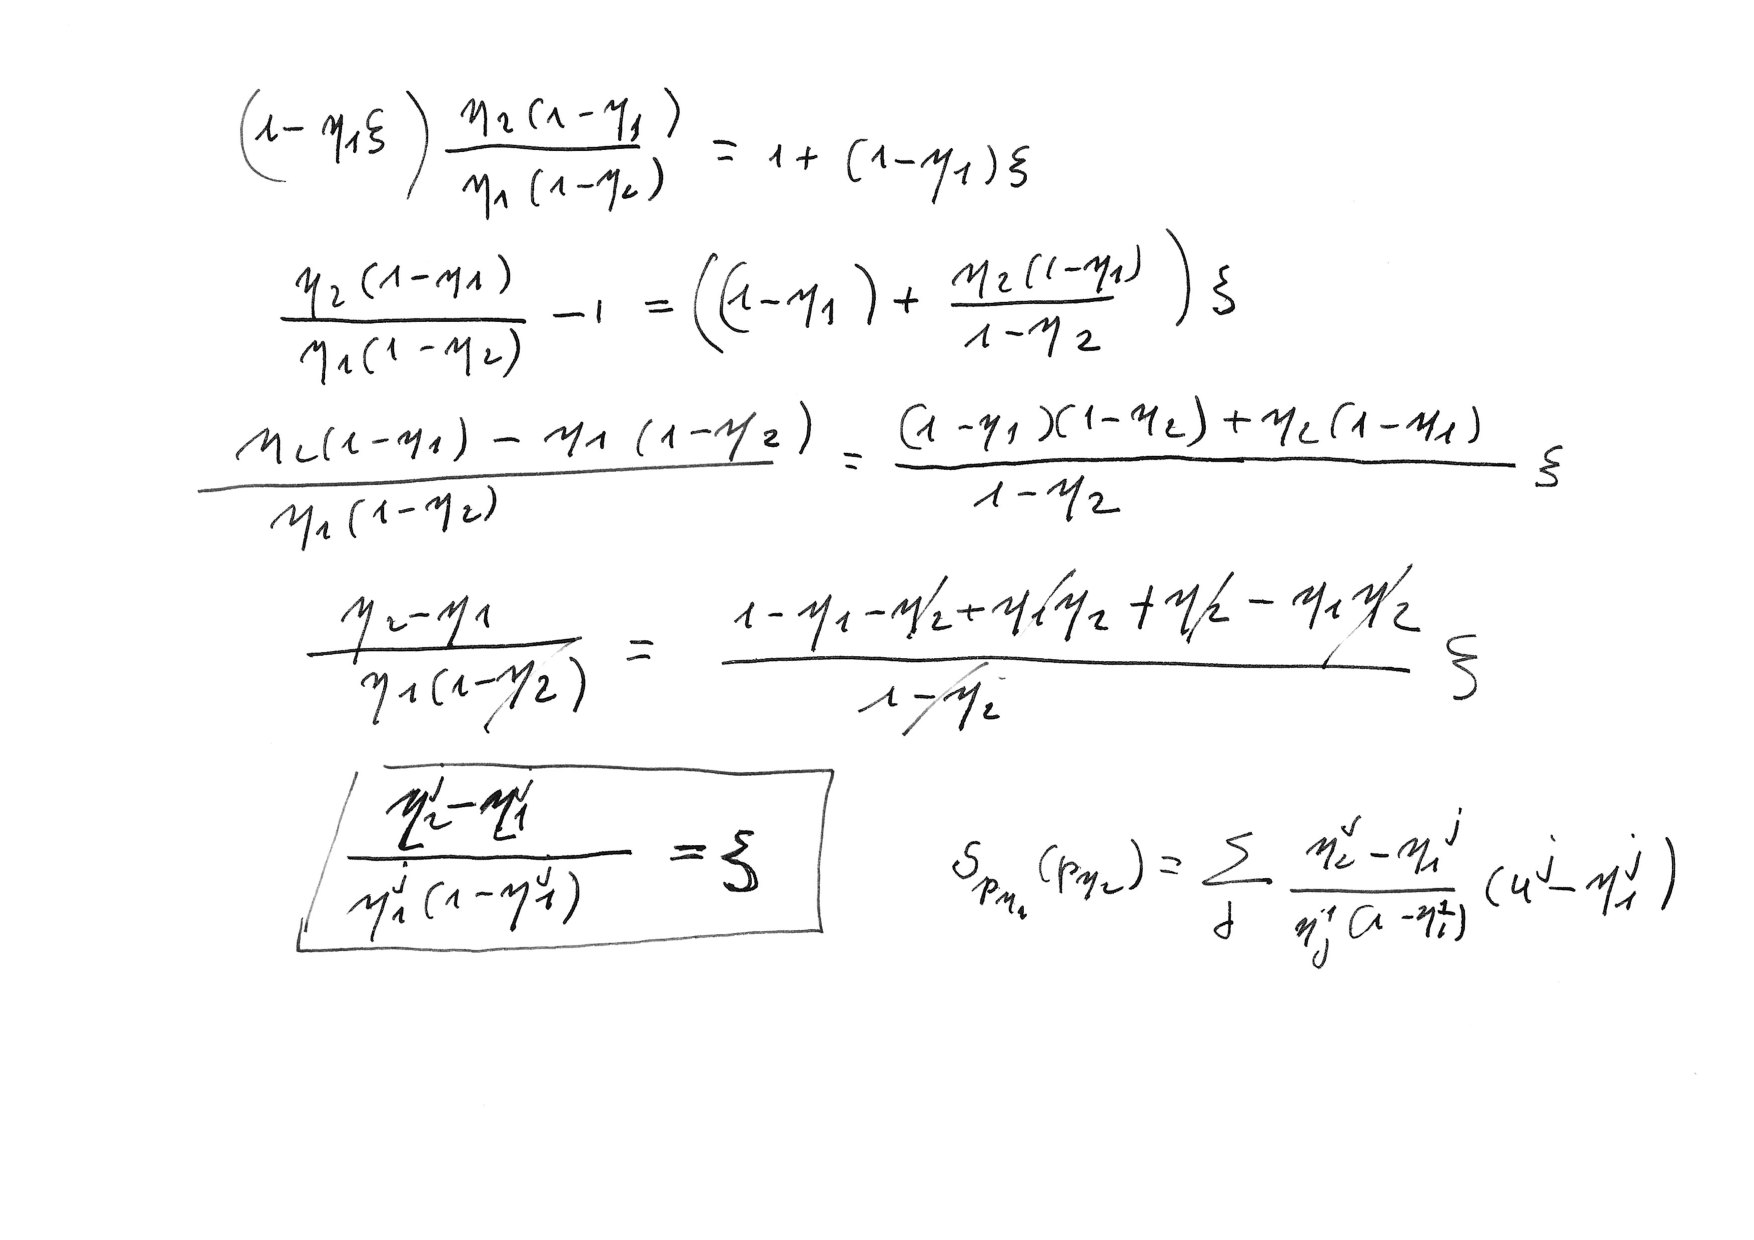
\includegraphics[width=\textwidth]{scans/scan-1.pdf}

 Let us check the parallelogram law. From \cref{eq:39a},
 \begin{multline}
   \label{eq:48}
   \sum_{j=1}^n \frac{\eta^j_2-\eta_1^j}{\eta_1^j(1-\eta_1j)}(u^j-\eta_1^j) + \mtransport {p_{\eta_2}}{p_{\eta_1}} \sum_{j=1}^n \frac{\eta^j_3-\eta_2^j}{\eta_2^j(1-\eta_2^y)}(u^j-\eta_2^j) = \\
   \sum_{j=1}^n \frac{\eta^j_2-\eta_1^j}{\eta_1^j(1-\eta_1^j)}(u^j-\eta_1^j) + \sum_{j=1}^n  \frac{\eta^j_2(1-\eta^j_2)} {\eta^j_1(1-\eta^j_1)} \frac{\eta^j_3-\eta_2^j}{\eta_2^j(1-\eta_2^j)}(u^j-\eta_1^j) = \\
   \sum_{j=1}^n \frac{\eta^j_3-\eta_1^j}{\eta_1^j(1-\eta_1^j)}(u^j-\eta_1^j) 
 \end{multline}

\subsubsection{Gradient and gradient flow}
\label{sec:gradient}

Let $F \colon \maxexpat V \to \reals$ be a scalar field. The gradient of $F$ is a section  $q \mapsto \Grad F(q)$ of the statistical bundle such that for all smooth curve $t \mapsto q(t) \in \maxexpat V$, that is, $q(t) = p_{\eta(t)}$ for some curve $t \mapsto \eta(t)$ in the space of expectation parameters, it holds
\begin{equation}
  \label{eq:gradient}
  \derivby t F(q(t)) = \scalarat {q(t)} {\Grad F(q(t))}{\velocity q(t)} \ .
\end{equation}

Let us write $\hat F(\eta) = F(q)$ and $\Grad F(q) = \sum_{j=1}^n \hat F_j(\eta) (u^j - \eta^j(t)$, provided $q = p_\eta$. From \cref{eq:32}, the velocity is
\begin{equation}
  \label{eq:55}
  \velocity q(t) = \sum_{j=1}^n \frac{\dot \eta^j(t)} {\eta^j(t))(1 - \eta^j(t))} (u^j - \eta^j(t)) \ .
\end{equation}

It follows from the expression of the inner product in \cref{eq:29} that 
\begin{multline}
  \label{eq:54}
  \derivby t \hat F(\eta(t)) = \scalarat {q(t)} {\Grad F(q(t))}{\velocity q(t)} = \\ \sum_{j=1}^n \eta^j(t)(1-\eta^j(t)) \hat F_j(\eta(t)) \frac{\dot \eta^j(t)} {\eta^j(t))(1 - \eta^j(t))} (u^j - \eta^j(t)) = \sum_{j=1}^n \hat F_j(\eta(t)) \dot \eta^j(t) \ , 
\end{multline}
that is
\begin{equation}
  \label{eq:58}
  \Grad F(p_\eta) = \sum_{j=1}^n \pderivby {\eta^j} \hat F(\eta) (u^j - \eta^j) \ .
\end{equation}

The gradien flow equation is $\velocity q(t) = - \Grad F(q(t))$, that is,
\begin{equation}
  \label{eq:61}
  \sum_{j=1}^n \frac {\dot\eta^j(t)}{\eta^j(t)(1-\eta^j(t))}(u^j - \eta^j(t)) = - \sum_{j=1}^n \pderivby {\eta^j(t)} \hat F(\eta) (u^j - \eta^j(t)) \ ,
\end{equation}
namely, in the expectation coordinates,
\begin{equation}
  \label{eq:62}
  \dot \eta^j(t) = - \eta^j(t)(1-\eta^j(t))\pderivby {\eta^j(t)} \hat F(\eta(t)) \ , \quad j=1,\dots,n \ .
\end{equation}

\begin{example}[Approximating a generic PF]  If $F$ is the KL divergence $\KL q \cdot$, $q \in \maxexpat {\set{0,1}^h}$,
\begin{multline}
  \label{eq:59}
  F(p_\eta) = \KL {q}{p_\eta} = \entropyof q - \expectat q {\log p_\eta} = \\ \entropyof q - \expectat q {\sum_{j=1}^n \log \frac{\eta^j}{1-\eta^j} u^j - \sum_{j=1}^n \log \frac 1 {1 - \eta^j}} = \\ \entropyof q - \sum_{j=1}^n \log \frac{\eta^j}{1-\eta^j} \expectat q {u^j}  + \sum_{j=1}^n \log \frac 1 {1 - \eta^j} \ ,
\end{multline}
then
\begin{gather}
  \label{eq:60}
  \pderivby {\eta^j} \KL {q}{p_\eta} =  - \frac 1 {\eta^j(1-\eta^j)}\left(\expectat q {u^j} - \eta^j\right) \ , \\
  \label{eq:60b}
  \Grad F(p_\eta) = - \sum_{j=1}^n\frac1{\eta^j(1-\eta^j)}\left(\expectat q {u^j} - \eta^j\right)(u^j - \eta^j) \ .
\end{gather}

Notice that $\Grad F$ is zero if, and only if, $\expectat q {u^j} = \eta_j$, $j = 1,\dots,n$. The equation for the gradient flow is
\begin{multline}
  \label{eq:56}
  \sum_{j=1}^n \frac {\dot\eta^j(t)}{\eta^j(t)(1-\eta^j(t))}(u^j - \eta^j(t)) = \\ 
  \sum_{j=1}^n\frac1{\eta^j(t)(1-\eta^j(t))}\left(\expectat q {u^j} - \eta^j(t)\right)(u^j - \eta^j(t))
\end{multline}
and, in the expectation coordinates,
\begin{equation}
  \label{eq:57}
\dot\eta^j(t) = \expectat q {u^j} - \eta^j(t) \ , \quad j=1,\dots,n \ ,   
\end{equation}
with solution
\begin{equation}
  \label{eq:63}
  \eta^j(t) = \expectat q {u^j} + (\eta^j(0) - \expectat q {u^j}) \euler^{-t} \ .
\end{equation}
\end{example}

\begin{example}[Linear model]
  The following example is inspired by the Raus et al paper.

  Let be given a matrix $A \in \reals^{m \times n}$ and a vector $b \in \reals^m$. Let us find the $p_\eta \in \maxexpat V$ such that the SSQ of the error in the linear model $Au=b$ is minimal,
  \begin{equation}
    \label{eq:64}
    \hat \eta \in \Argmin_\eta \expectat {p_\eta}{\normof{Au - b}^2} \ .
  \end{equation}
\end{example}

\begin{example}[Linear syntesis]
  Let $A$ be an $m \times n$ matrix and xonsider the random variable $y = Au$. The distribution of $y$ is characterised by
\end{example}

\begin{equation}
  \label{eq:65}
  \bar s_p(q) = \transport p {\bar p} s_p(q)
\end{equation}
END


% \bibliographystyle{amsplain}
\bibliographystyle{plainnat}
\bibliography{tutto}

\end{document}

%%% reflex-default-bibliography: ("./")
%%% Local Variables:
%%% mode: latex
%%% TeX-master: t
%%% End:
